\documentclass[11pt,pdftex]{article}

\usepackage{deauthor}
\usepackage{times}
\usepackage{xcolor}
\usepackage{hyperref}
\usepackage{graphicx}
\usepackage{bmpsize}
\usepackage{makecell}

% OTHER PACKAGES GO HERE
% List all packages used in your article, eliminating duplicates
% Do not include packages not actually used in your paper
% DO NOT COMMENT OUT PACKAGES, REMOVE THEM
% Ensure that your paper does not include the packages below
% geometry, subfigure, enumitem

% COMMANDS GO HERE
%please list all commands used in your paper, eliminating duplicates

% Your paper submission must be in a folder named with the
% contact author name.

\graphicspath{ {submissions/Sudakshina2023/figs/} }

\begin{document}


\title{Bringing Order to Chaos: Conceptualizing a Personal Research Knowledge Graph for Scientists}
\author{Prantika Chakraborty\textsuperscript{$\dagger$}, Sudakshina Dutta\textsuperscript{$\ddagger$}, Debarshi Kumar Sanyal\textsuperscript{$\dagger$}, 
\\
Srijoni Majumdar\textsuperscript{*}, Partha Pratim Das\textsuperscript{**}
\\\\
\textsuperscript{$\dagger$}Indian Association for the Cultivation of Science, Kolkata-700032, India
\\
\textsuperscript{$\ddagger$}Indian Institute of Technology Goa, Ponda-403401, India\\
\textsuperscript{*}University of Leeds, Leeds
LS2 9JT, UK\\
\textsuperscript{**}Indian Institute of Technology Kharagpur, Kharagpur-721302, India,\\ 
\textsuperscript{**}Ashoka University, Haryana-131029, India\\
\texttt{intpc@iacs.res.in}, \texttt{sudakshina@iitgoa.ac.in},\\
\texttt{debarshi.sanyal@iacs.res.in}, 
\texttt{s.majumdar@leeds.ac.uk}, \\
\texttt{ppd@cse.iitkgp.ac.in}
}


\maketitle

\begin{abstract}
Research and work-related information is often manifold for a scientist, and the absence of an organizing system may impede their research.  Information that holds immense personal interest and importance to a scientist may not be relevant to other users, yet it must be easily accessible to the scientist to enhance their productivity. We aim to address the need for such a system with our proposal of a knowledge graph for scientists, termed the \textit{Personal Research Knowledge Graph} (PRKG). To identify the components of a PRKG, we interview scientists at an academic institution for higher education and research regarding the issues that the presence of a PRKG could solve. We translate the scientists' requirements into separate KGs, collectively known as the `Vitamins of PRKG', and discuss  methods for data acquisition to construct and maintain the PRKG. A smart virtual agent is proposed as a medium of interaction between the user and the PRKG. We also outline future research tracks, including those focused on maintaining the PRKG and protecting personal data and privacy.
\end{abstract}

\section{Introduction} \label{prantika_sec:intro}
In an ever-expanding digital universe, scientists often find themselves entangled in the deluge of data necessary for their day-to-day professional activities. Instead of aiding in research work, the abundance of such data may, counter-intuitively, hamper it. Manually organizing all this information is a time-consuming activity that one might not always be eager to undertake. This brings in the requirement of a Personal Information Management (PIM) system that will aid in the collection of data, processing of the data into relevant information, and storage and eventual use of the information, with a strong emphasis on security and privacy \cite{jones2007personal}. 

In the world of PIM, researchers use abstractions such as  \textit{information type}, \textit{information item}, \textit{personal space of information} and \textit{personal information collection}  \cite{jones2017personal,jones2007personal}. An \textit{information type} or \textit{information form} denotes the mode (including the supporting applications) in which information is available and exchanged, such as paper-based letters, e-mails, and web pages, whereas an 
\textit{information item} denotes the encapsulation of  
information in a persistent form that can be managed (e.g., stored and transmitted), such as an individual e-mail message. In the context of object-oriented programming, an information item corresponds to an object and the information type of the item maps to its class. Information can be \textit{personal} to a user in several ways, which may be overlapping. In particular, a user's personal information includes information controlled or owned by the user, about the user, directed to the user, sent/posted/shared by the user, experienced by the user, or potentially relevant or useful to the user \cite{jones2017personal}. An individual has a single \textit{personal space of information (PSI)}, which includes all information items that they consider personal. \textit{Personal information collections (PICs)} are personally managed subsets of a PSI; an example is a folder containing downloaded research papers. Unlike an individual's  PSI, which can be enormous in size, a PIC is smaller and, therefore, can be effectively managed. PIM involves activities to manage the PICs of a user with an aim to create, use and maintain a mapping between the needs of the user and their personal information.  

Over the years, several PIM tools have been developed to assist users in organizing, maintaining, and utilizing their information items for various purposes.  Concepts such as the Semantic Desktop \cite{sauermann2005overview,breitman2007semantic}, which suggested the use of Semantic Web technologies \cite{berners2001semantic} to organize the information items on a user's desktop and integrate them with resources on the Web for an enhanced user experience in accessing and sharing personal information, have had a significant impact. 
The Semantic Desktop concept has evolved into the Social Semantic Desktop, as seen in frameworks like NEPOMUK \cite{groza2007nepomuk}, SemanticLIFE \cite{ahmed2004semanticlife}, and SocialLIFE \cite{vo2014sociallife}. Recent efforts for personal information management have been in the form of mind-mapping software like TheBrain \footnote{\url{https://thebrain.com/}} where one can store a network of interconnected thoughts and ideas, capture their evolution, visualise them, and search over them. The Solid Pod project \footnote{\url{https://solidproject.org/}}, led by Sir Tim Berners-Lee, offers users the opportunity to securely store their personal data in shareable data stores known as ``pods`` and to have complete control over their data and access to it. 

\subsection{Information Management for a Scientist}
A scientist needs to handle a large volume of information, which can be segregated into three main categories:
\begin{itemize}
    \item \textit{Research-related}: This information is related to the research activities of scientists and includes scholarly literature they reference for their work, the various tools and methods they employ, as well as upcoming events such as conferences and workshops in their respective fields. Scientists may also wish to capture summaries of meetings with collaborators about their work and extract useful information from these interactions. Moreover, scientists working in academic institutions, such as universities, typically teach courses in addition to handle their research responsibilities; therefore, they must also manage teaching-related information.
    
    \item \textit{Administrative}: A scientist or faculty member frequently participates in various administrative councils and needs to keep track of the developments of such councils and their meetings.
    
    \item \textit{Laboratory-related}: Managing a laboratory is a common aspect of a scientist's responsibilities. Storing salient information about laboratory equipment and resources may simplify access and auditing processes. 
\end{itemize}

Maintaining the aforementioned types of information in a structured and organized manner is often a challenging task for a scientist and can hinder their research work substantially. Having a PIM system makes storing and accessing such information less time-consuming, thereby enhancing the productivity of scientists.

\subsection{Personal Knowledge Graph}
Knowledge graphs (KGs) have been enjoying much popularity in recent times as a means for storing information in an organized manner \cite{ji2021survey,chaudhri2022knowledge}. A KG can be formally defined \cite{ehrlinger2016towards} as $\mathcal{G} = \{\mathcal{E}, \mathcal{R}, \mathcal{F}\}$. $\mathcal{E}$ denotes the set of entities, $\mathcal{R}$ denotes the set of relations, and $\mathcal{F}$ denote the set of facts, where each fact is a triple $(h, r, t)$ such that $h \in \mathcal{E}$, $t \in \mathcal{E}$ and $r \in \mathcal{R}$. 
A personal knowledge graph (PKG), proposed by Balog and Kenter  \cite{balog2019personal}, is a KG that is relevant to a particular user but may not be useful to others. The primary purpose of the PKG is to support the delivery of services that are customized particularly to its owner. 
Balog and Kenter \cite{balog2019personal} initially introduced the concept of a PKG with the following definition: 
\begin{itemize}
    \item[] \textbf{Definition 1:} A PKG is `a resource of structured information about entities \textit{personally related to its user}, their attributes and the relations between them'.
\end{itemize}
They model a PKG as a ``spider-web" like structure with a central node representing the user and all the other nodes connected to the central node, as shown in figure \ref{fig:pkg}.
In a more recent work co-authored by Balog  \cite{skjaeveland2023ecosystem}, a PKG is redefined as follows:
\begin{itemize}
    \item[] \textbf{Definition 2:} A PKG is a `a knowledge graph (KG) where a single individual, called the owner of the PKG, has (1) full read and write access to the KG, and (2) the exclusive right to grant others read and write access to any specified part of the KG.' 
\end{itemize}
The second definition differs from the first one in that the entities of the PKG \textit{need not} be directly connected to the owner.
Lately, several PKGs have been proposed and developed to assist users in the field of health, finance, education and research \cite{Chakraborty2023comprehensive}. For example, a PKG containing an individual's health information may be useful for their dietary planning and medical checkups \cite{seneviratne2021personal}. A PKG is created and owned by the user whose personal information is held in it; this ensures the privacy of the data.  
\begin{figure}[!htbp] 
    \centering
    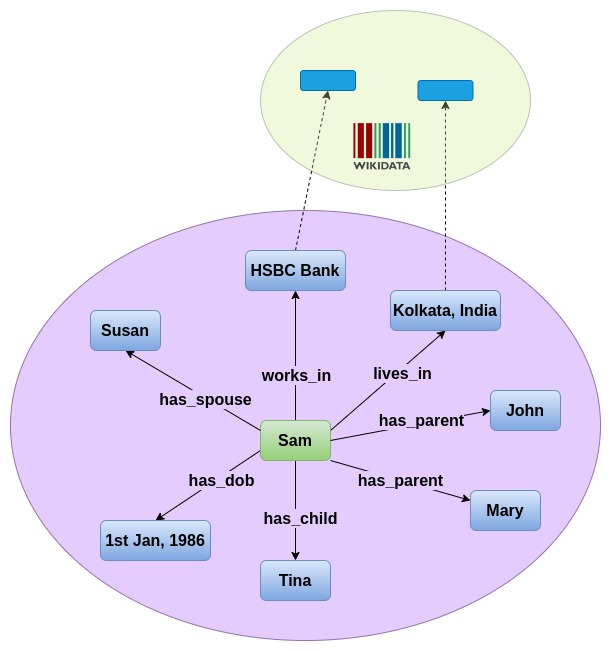
\includegraphics[width=0.5\textwidth]{submissions/Sudakshina2023/figs/PKG.jpg}
    \caption{An example of PKG containing Sam's personal data \cite{Chakraborty2023comprehensive}.}
    \label{fig:pkg}
\end{figure}

PIM focuses on \textit{activities} related to managing the personal information of an individual, but the emphasis of this paper is on PKG which is a \textit{data structure} to store the individual's personal information. While PIM deals with information items, PKG handles more granular units which are facts or triples extracted from information items. Therefore,  tools for creation and maintenance of traditional PIM systems are not directly applicable to manage PKGs. 

\subsection{Our Proposal}
In this position paper, we focus on PKGs for scientists; we call it PRKG -- a shorthand for \textit{P}ersonal \textit{R}esearch \textit{K}nowledge \textit{G}raph. 
PRKG for an individual researcher will be owned and maintained by the researcher. 
Formally, a PRKG is defined as $\mathcal{P} = \{u, \mathcal{G}\}$ where $u$ denotes the owner of the PRKG and $\mathcal{G} = \{\mathcal{E}, \mathcal{R}, \mathcal{F}\}$ denotes the KG containing the `facts' in the PRKG. To represent the owner as a node in the PRKG, a fact in which the owner is one of the entities is created. Such a fact could be the following $(u, owns, p)$ where $u, p \in \mathcal{E}$, $owns \in \mathcal{R}$, and $p$ represents the current PRKG. Following \textbf{Definition 2}, we do not require all facts or triples to be connected to the owner node $u$.

In order to leverage the knowledge reserved in the PRKG, an intelligent virtual agent may be designed to access the PRKG, serving as a conduit for interaction between the scientist and their PRKG. The agent will be capable of deducing essential information based on the scientist's needs or even act proactively, and can also modify the PKG by incorporating new information or updating existing data. Note that the PRKG mitigates the cold start problem that services like personalized recommendation systems encounter when bootstrapping for a new owner.

Fundamental questions on the design and use of a PRKG pertain to the identification of the information that should be included in it, the representation of structured information within a PRKG, methods to populate and maintain the graph, and the proper utilization of the PRKG to assist the owner.
The remainder of the paper is organized as follows. Section \ref{prantika_sec:requirements} summarises the various requirements highlighted by researchers for their PKGs. Section \ref{prantika_sec:prkg} discusses our proposal for the Research PKG in detail whereas Section \ref{prantika_sec:acquisition} discusses methods for data acquisition for the creation of PRKGs and issues related to PRKG maintenance. Section \ref{prantika_sec:interact} suggests methods in which a scientist can interact with the PRKG. Section \ref{prantika_sec:future} discusses future research directions for the field, and Section \ref{prantika_sec:conclusion} concludes the paper. For the rest of the paper, the terms ``owner'' and ``user'' are used synonymously and assumed to refer to a ``scientist'' who owns (and therefore, creates and manages) the PKG we will discuss.


\section{Content in a PRKG: What do researchers say?} 
\label{prantika_sec:requirements}
We interviewed six researchers specializing in chemistry, physics, and biology at the premier research institution where the first author works. We inquired about the information they would prefer to store in a PRKG, how they plan to use that information, and, if presented with an AI-bot powered by this database, what expectations they would have from it. One observation that we concluded was that researchers mostly looked at the PRKG as a database of research-related information.

\textit{Research paper metadata: }The information that all researchers wanted to store in the PRKG includes metadata such as the title, author names, year and venue of publication, inferred keywords, and custom user-guided tags for the papers they read. Scientists commonly download papers and save them on their desktops without systemically categorizing them, and later encounter difficulty in retrieving specific articles. The researchers would like to have these information available in the PRKG so that a desktop search engine or a chatbot could answer related queries. Some researchers wanted to store annotations they add to a paper or the paper's main findings extracted by a smart AI-based application. 

\textit{Email metadata and summary: }Some of the researchers have told us that they receive numerous emails every day in their official email id, and more than half of them are unimportant or close to spam. Consequently, there is a risk that critical emails, such as those seeking project positions, may get buried and go unattended. They wished to have the important emails automatically discerned and indexed in the PRKG so that applications can generate alerts for them. These emails could range from upcoming meetings or manuscript submission deadlines to those that require long-term and situation-dependent reminders. For instance, when a researcher advertises a project position, they may want to be reminded of a query email received for a project position long ago. 

\textit{Event and schedule information: }In order to generate regular reminders for various tasks like manuscript submission, paper review, etc. researchers wanted to store the deadlines for such tasks in the PRKG. Information about meeting dates and times, exam schedules, project timeline could also be stored in the PRKG as suggested by the researchers.

\textit{Research meeting/discussion summary: }Another category of knowledge that all the researchers wanted to curate in the PRKG is that gleaned from research meetings, potentially in the form of concise summaries. All the researchers we interviewed supervise Master's and PhD students, and have frequent academic discussions with them. Many new ideas and questions come up during these internal meetings and most escape documentation. The researchers wanted the PRKG to remember them so they could be revisited later. For instance, unanswered questions or negative results discussed in a meeting should be documented as they might motivate novel investigations in the future. Some of the researchers mentioned that the meeting attendees often use a mix of English and a local language like Bengali, and it would be helpful if the necessary information could still be extracted and stored in the PRKG.

\textit{Financial information (Project grants and lab equipment): }Researchers who make extensive use of lab equipment also wanted to store their equipment-related information, for example, of servers and other high-end devices, in the PRKG. These information could be extracted from purchase documents. An AI-bot might use this information to perform periodic audits of the devices and advise maintenance activities. One researcher who aims to build an advanced lab desired to store information from quotations for various lab equipment so that applications could easily compare them and recommend the best equipment to purchase. Another suggestion was to store information related to project grants and fund utilization since they are often difficult to remember and track, yet need to be frequently accessed. 

\textit{Journal/Conference information: }One researcher mentioned having personal preferences regarding journals and conferences, desiring search results (from the web or desktop) to be ordered based on these preferences. These preference or trust lists could be stored in the PRKG. Some researchers desired the PRKG to be utilized for generating customized recommendations for articles and publication venues that match their interests. 

\textit{Information on collaborations: }Another researcher highlighted having multiple collaborations, and for information about collaborators (automatically extracted from emails) to be stored in the PRKG. This researcher even discussed the possibility of assigning priorities to these collaborations, establishing a partial order that could be used to customize email alerts and schedule meetings. The PRKG should store this personal priority list for the researcher. The researcher mentioned that they might even define a priority over the collaborations; this partial order might be harnessed to customize email alerts and schedule meetings. The PRKG should store this priority list, which is completely personal to the researcher.

\textit{Experiment-related information: }Another researcher wanted more fine-grained information from papers. As a microbiologist, he wanted details about chemicals and apparatus from papers to be extracted and stored in the knowledge graph. This information could be valuable for learning about and purchasing improved versions of the materials used in experiments. This researcher also wanted the PRKG to have access to lab notebooks to capture fine-grained information about experiments they conduct. This information could be valuable in tracing any discrepancies in experimental results arising from frequently overlooked differences in experimental settings. They believe that this approach might contribute to addressing the replication crisis in biology to some extent. 

\textit{Course-related information: }Researchers affiliated to educational institutions have to undertake the responsibility of teaching a designated number of courses. One of the researchers we interviewed emphasized the potential of storing curated information from a course's schedule, outline, and materials (textbooks, articles, papers, presentations, etc.) in the PRKG. The researcher also noted that they acquire information about courses of interest taught at leading universities by browsing the Internet, and this information may be stored in the PRKG. The AI-bot may use this information to help the researcher design their own courses.

\textit{Role of AI-bot: }In response to our question on the expectations from an AI-bot capable of engaging in conversational dialogues with scientists, one researcher said they wanted the agent to assist new research scholars in generating the first iteration of the literature review. Another researcher wondered if the agent could help them formulate new research questions given the experimental data and sample questions already formulated. Interestingly, the latter requirement where an AI system helps to \textit{do} science is still a work-in-progress for the AI community. A researcher wanted the bot to be integrated with simple science tools, for example, to convert a table of values from one unit to another, when instructed to do so in natural language; such a tool is useful in meetings with funding agencies and collaborators where quick answers are expected. Another researcher wished the agent to automate the submission of travel and dearness allowance-related documents, given a short prompt from the researcher and access to their or relevant documents. Another capability that some of the scientists mentioned is to automatically generate a TODO list, which includes alerts for meetings but potentially encompasses various other activities. 

\section{Building Blocks of a PRKG} 
\label{prantika_sec:prkg}
We now outline a blueprint for a Personal Research Knowledge Graph (PRKG) owned and managed by a science researcher. A similar proposal was made regarding a PKG for researchers in \cite{chakraborty2022} where the central node represents the owner, and various entities related to the owner's research aspects are connected to it. 
However, the current proposal does not require the owner to be linked to all the facts. Further, we organize the PRKG as a collection of several knowledge graphs (KGs), each originating from a specific kind of knowledge source, and together referred to as the \textit{vitamins of PRKG} for their first letters are reminiscent of vitamins, as shown in Figure \ref{fig:vitaminsPRKG}. Table \ref{tab:requirements_PRKG} shows how particular information that the researchers want to store in their PRKG, as discussed in Section \ref{prantika_sec:requirements}, can be mapped onto the different individual KGs that are described as follows:

\begin{figure}[!htbp]
    \centering
    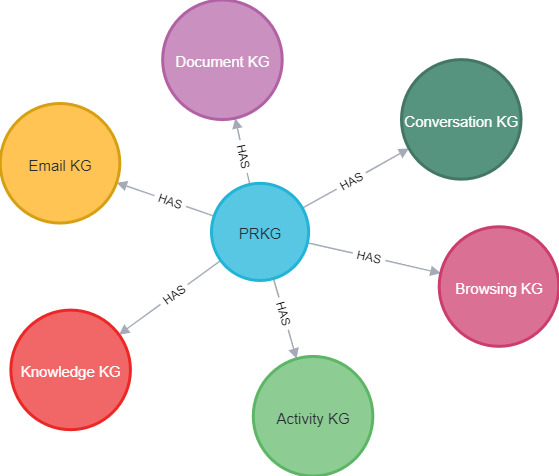
\includegraphics[width=0.68\linewidth]{submissions/Sudakshina2023/figs/PRKG_Components.jpg}
    \caption{Vitamins of PRKG}
    \label{fig:vitaminsPRKG}
\end{figure}

\begin{itemize}
    \item \textit{\textbf{A}ctivity KG}: A KG that will contain information regarding the owner's activities, such as scheduled meetings and events, will be called the \textit{Activity KG}. This KG will help the user in setting reminders for upcoming events like meetings, talks, conferences, journal submissions, lectures to be taken, etc. The KG will have access to the owner's system logs, calendars, and digital planners for regular updates. 
    \item \textit{\textbf{B}rowsing KG}: A KG that contains the owner's browsing history-related data will be referred to as the \textit{Browsing KG}. This may include web search logs, encompassing scholarly search engines like Google Scholar and academic social networks like ResearchGate, from which the owner's current research interests can be inferred. Web logs can also help inform recommendations, for example,  conference pages visited may provide insights regarding conferences that the owner might like to attend in the future.
    \item \textit{\textbf{C}onversation KG}: A KG that contains knowledge inferred from conversations over applications 
    like WhatsApp and Skype will be called the \textit{Conversation KG}. Knowledge drawn from transcripts of meetings held online over video-telephonic applications like Zoom may also be incorporated in this KG. The goal is to store summarised knowledge from these conversations and meetings, that may range from updates on current works to ideas for new projects.
    
    \item \textit{\textbf{D}ocument KG}: Documents related to the owner's research pursuits, teaching activities, lab equipment, and administrative affairs are stored either locally on the user's machine or in remote storage owned by the user. A \textit{Document KG} will capture knowledge extracted from the above sources. For example, it may contain the metadata from papers being read by the user, the timetable of the course offered by the user in the current semester, essential information extracted from recent office memorandums, and details of recent purchases. An expanded Document KG could also include multimedia files like images, audio and videos. 
    
    \item \textit{\textbf{E}mail KG}: A KG that will hold information gleaned from a user's work-related emails will be referred to as the \textit{Email KG}. This KG will extract relevant entities from email chains that a user holds with his collaborators. This includes basic information regarding the collaborators, like their affiliations and contact details. Identifying potential collaborators and the main topics of discussion with them can also enhance the Email KG. 
    \item \textit{\textbf{K}nowledge KG}: The information about the user that they themselves provide will be stored in \textit{Knowledge KG}. It potentially includes the user's current affiliations, research interests, and personal beliefs and preferences (say, about fellow researchers in their community or books on a particular topic). 
  
\end{itemize}

\begin{table}
    \centering
\caption{Mapping researchers' requirements, as discussed in Section \ref{prantika_sec:requirements}, to the various building blocks of a PRKG, as discussed in Section \ref{prantika_sec:prkg}}
\label{tab:requirements_PRKG}
    \begin{tabular}{l l l} \hline 
         \textbf{Researchers' requirements}& \textbf{Requirement frequency by user}& \textbf{Relevant PRKG sub-graph}\\ \hline 
         Research paper metadata& 6& Document KG\\
         Email metadata and summary& 6 & Email KG\\ 
         Event and schedule information& 5 & Activity KG, Email KG\\ 
         Research meeting/discussion summary & 4 & Email KG, Conversation KG\\ 
         \makecell[l]{Financial information including project \\  grants and lab resources' quotations}& 3 & Document KG\\ 
         Journal/conference information& 3 & Knowledge KG, Browsing KG\\ 
         Information on collaborations & 2 &  Email KG, Conversation KG\\
         Experiment-related information & 1 & Document KG \\
         Course-related information &1 & Document KG, Browsing KG \\ \hline
    \end{tabular}
    
    
\end{table}

It is worth noting that these integrant KGs are not disjoint KGs. For instance, a person who undertakes frequent collaborations with the user will be present in both the Document KG as a co-author and the Email KG as a collaborator, and will be modeled by the same node. This can be achieved by entity disambiguation and linking.

An important question is: at what granularity should information be stored in the PRKG? For an Activity KG, one can extract precise details of a scheduled meeting, like the topic, time, venue, and invitee list from the user's calendar. But in the case of a Conversation KG or an Email KG, storing a free-form textual summary of a conversation chain as a text blob may be more practical because it is hard to define \textit{a priori} the granular entities to extract from messages and even harder to train an entity extractor for the task while state-of-the-art tools for text summarization and question-answering from unstructured text display superb performance, thanks to large language models. Meeting summaries may be utilized by external applications, such as neural question-answering systems, to answer more specific user queries. Nevertheless, if it is possible to define fine-grained entities like collaborator names, conferences (visited by the user), and journals (to which the user submits papers), they should be identified from the information item and incorporated into the relevant sub-KG. 

Entities and relations may be stored as Resource Description Framework\footnote{\url{https://www.w3.org/RDF/}} \cite{miller1998rdf} (RDF) triples of the type $ \langle subject-predicate-object \rangle $. A desirable aspect of this information storage is the inclusion of \textit{provenance} of the RDF triples, which helps identify the source of the information and the process by which it was extracted. This is essential for determining the quality of information extracted and the correctness and trustworthiness of the process used to extract this information \cite{sikos2020provenance}.

\begin{figure}[!htbp]
    \centering
    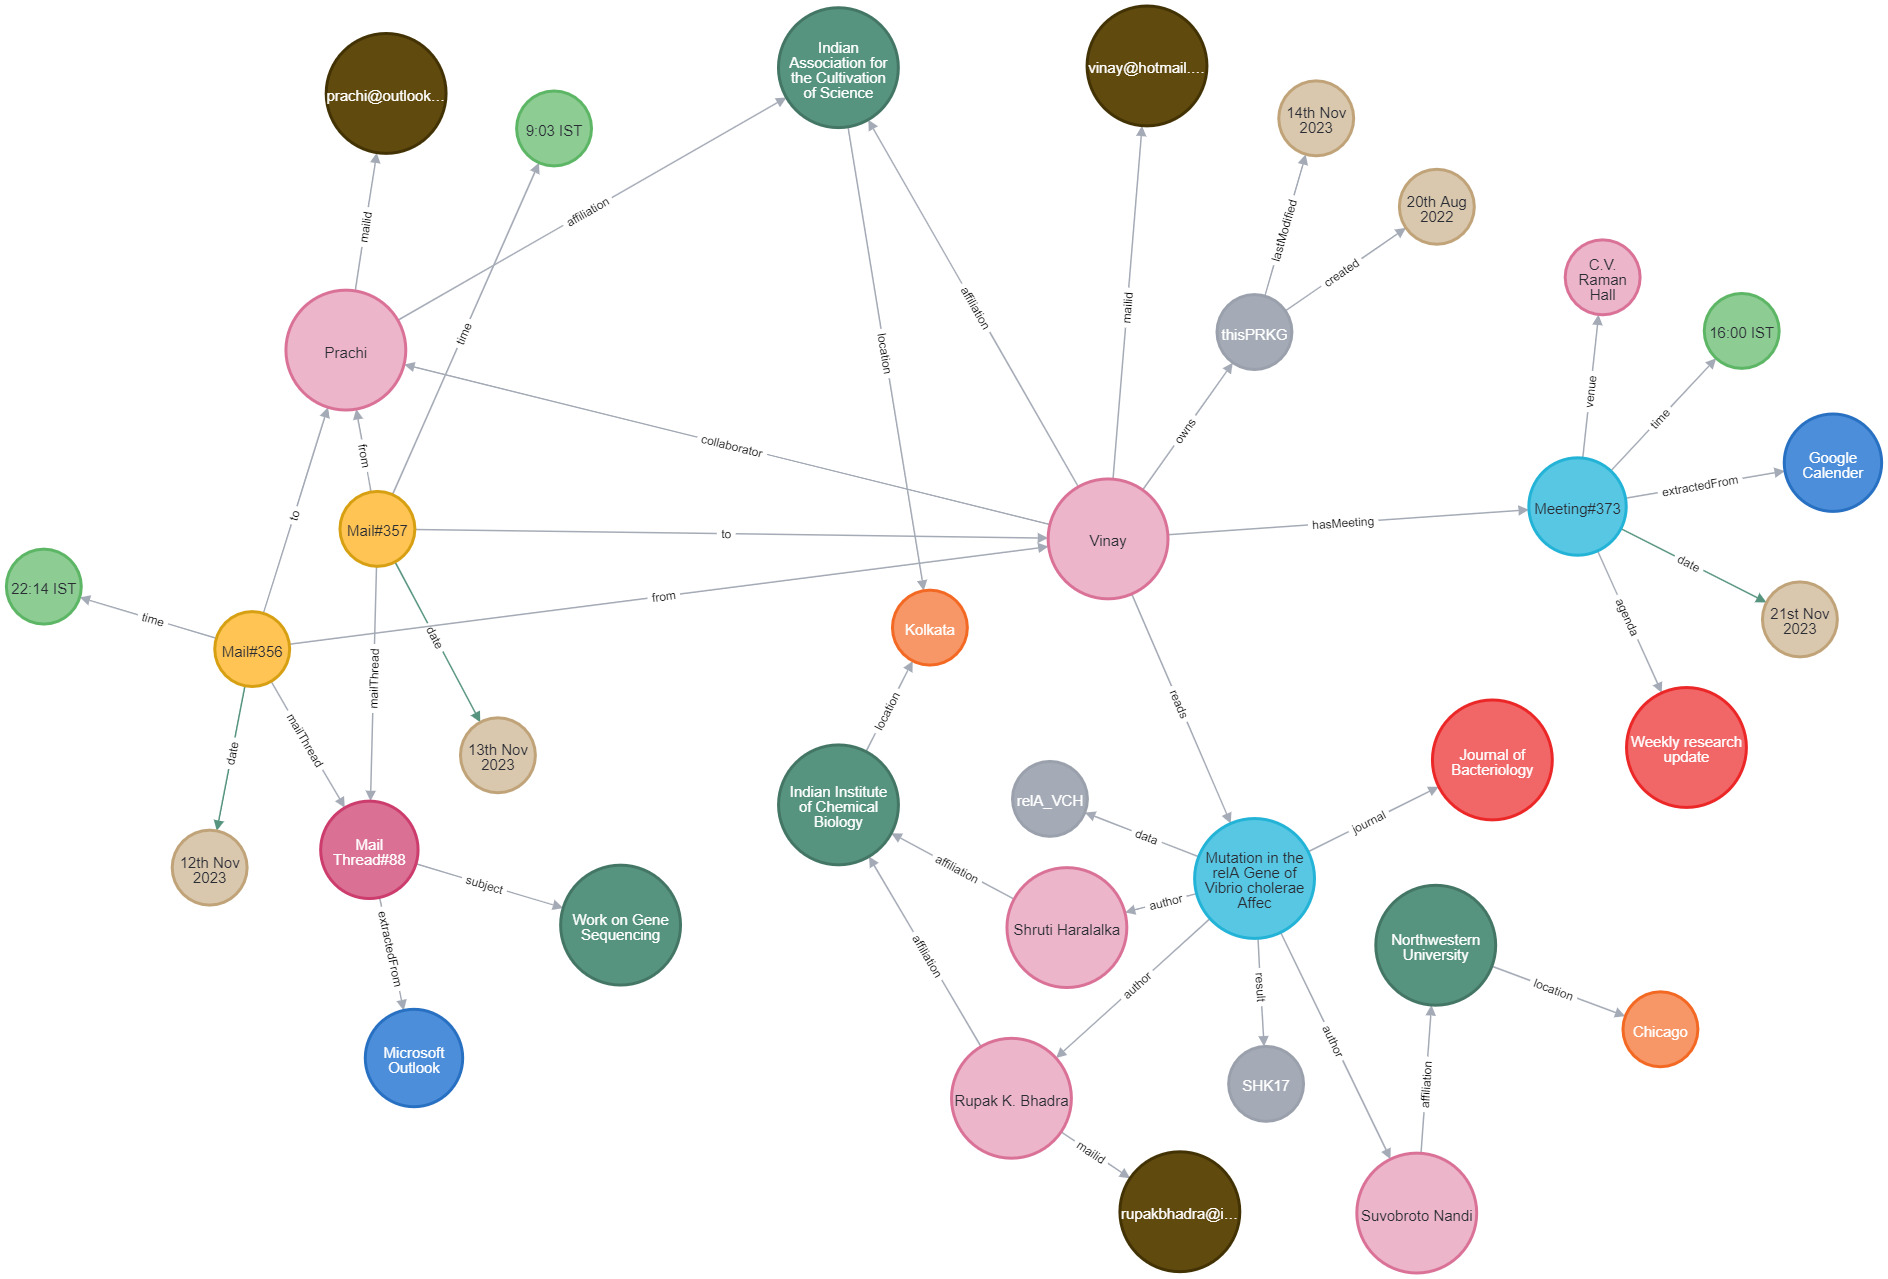
\includegraphics[width=0.9\textwidth]{submissions/Sudakshina2023/figs/PRKG_new.jpg}
    \caption{Snippet of a PRKG}
    \label{fig:prkg}
\end{figure}

\paragraph{Illustration of a PRKG:} Figure \ref{fig:prkg} shows a snippet of a PRKG whose owner is Vinay, a researcher. This PRKG is a sample comprising triples of the Activity KG, the Document KG and the Email KG. Although conceptually we have segregated the PRKG into smaller divisions based on the source of the knowledge, the actual PRKG we have created is a heterogeneous mixture of triples from all the smaller KGs. The graph reveals that Vinay is scheduled to have a meeting (specifically, \textit{meeting 373}) on \textit{21st November 2023} at \textit{4:00 pm IST} at the \textit{C.V. Raman Hall}. The meeting's agenda is his \textit{Weekly research update}. This is an excerpt of the Activity KG of his PRKG. We also see how Vinay's communication with \textit{Prachi}, who is a possible collaborator, via mail has been captured by the Email KG. Prachi's email ID and affiliation have been stored as information from the emails exchanged between Vinay and Prachi. The summary of their email thread will also be stored in the Email KG but has been excluded from this figure for brevity. This PRKG also stores metadata from papers that Vinay downloads for reading. One such paper is titled  ``Mutation in the \textit{relA} Gene of \textit{Vibrio cholerae} Affects In Vitro and In Vivo Expression of Virulence Factors''  \cite{haralalka2003mutation}, written by \textit{Shruti Haralalka, Suvobroto Nandi,} and \textit{Rupak K. Bhadra}, and published in \textit{Journal of Bacteriology}. Additional  information about the authors, such as their current affiliation and contact details, is extracted from the paper. This PRKG was created using the Enterprise Edition of Neo4j 5.2.0, which is provided with Neo4j Desktop version 1.5.9. The graph is best viewed when zoomed in digitally.



\section{Data Acquisition and PRKG Maintenance} 
\label{prantika_sec:acquisition}
We introduced six constituent KGs in the previous section. The knowledge captured in these KGs come from diverse sources spanning multiple devices. We envisage that custom tools will be written to extract entities and relations of interest from these sources to populate the corresponding KGs.  LLMs may also be prompted to extract this information from various sources.

As an example, consider the Activity KG. Calendar services like Google Calendar and Microsoft Outlook Calendar have become irreplaceable when it comes to keeping track of a user's scheduled events like meetings and lectures. Currently, there are a number of APIs, like \textit{Make}\footnote{\url{https://www.make.com/en/api-documentation}}, \textit{Notion}\footnote{\url{https://developers.notion.com/}}, and \textit{REST}\footnote{\url{https://tinyurl.com/ibmRestApi}}, that can sync information from such calendars and store them in a database that will be eventually used to create the Activity KG. Note that most schedules and deadlines are first programmatically extracted from emails and then pushed to the user's calendar. Similarly, a Browsing KG can simply track the user's browsing activities, remember visited websites, and incorporate derived knowledge like research interests, frequently visited university websites, and commonly used online tools. 

For the other KGs, namely Conversation KG, Document KG, and Email KG, we envisage an application that first identifies the precise resources to be harvested for inclusion in the PRKG. Once that information is available, the application analyzes the resources to extract relevant knowledge. As a concrete example, consider an application that allows the PRKG owner to indicate which emails should be parsed for inclusion into the Email KG. This application may \textit{learn} to suggest emails that should be included, and once the user agrees, it can proceed to process them. Similarly, the user may explicitly indicate folders or files should come under the scope of the Document KG. As regards the structured information to be extracted from these resources, they are of two kinds: (1) \textit{metadata}:  consider these examples: (a) for emails in Email KG, the sender, recipients, subject and  date may be extracted; (b) for research papers in  Document KG, the title, author names, keywords, publication venue, and publication date are salient fields; (2) \textit{deep data}: this includes an analysis of the content of the resource; examples of such information are (a) for emails with collaborators, the collaborators' names and affiliations, and keywords that capture the collaboration area; (b) for downloaded research papers, the problem, methods used, and essential findings. While the metadata fields may be easy to identify for a specific information type, defining the deep data fields is  challenging and may potentially depend on the user's interest. Machine learning models that can \textit{learn} new entity types from a few user-provided examples may be useful here.

PKGs differ from general-purpose KGs in that they capture entities and relations that are personal to the user. A user's personal preferences and activities evolve over time, making old information in the PKG useless for most applications. This volatility of information and the consequent requirement for PKG maintenance are important characteristics of a PKG. In case of Activity KG and Browsing KG, these aspects are highly visible; stale information should be flushed out to avoid unnecessary memory consumption. However, for conversations, emails, and arguably documents, it might not be prudent to delete old facts as the user might like to revisit them in future. To capture the freshness of a triple, the PRKG might associate temporal information like the creation date and the last access date of the triple. This temporal information might be useful for applications that use the PRKG to deduce the owner's current behavioural characteristics.


\begin{figure}[!htbp]
    \centering
    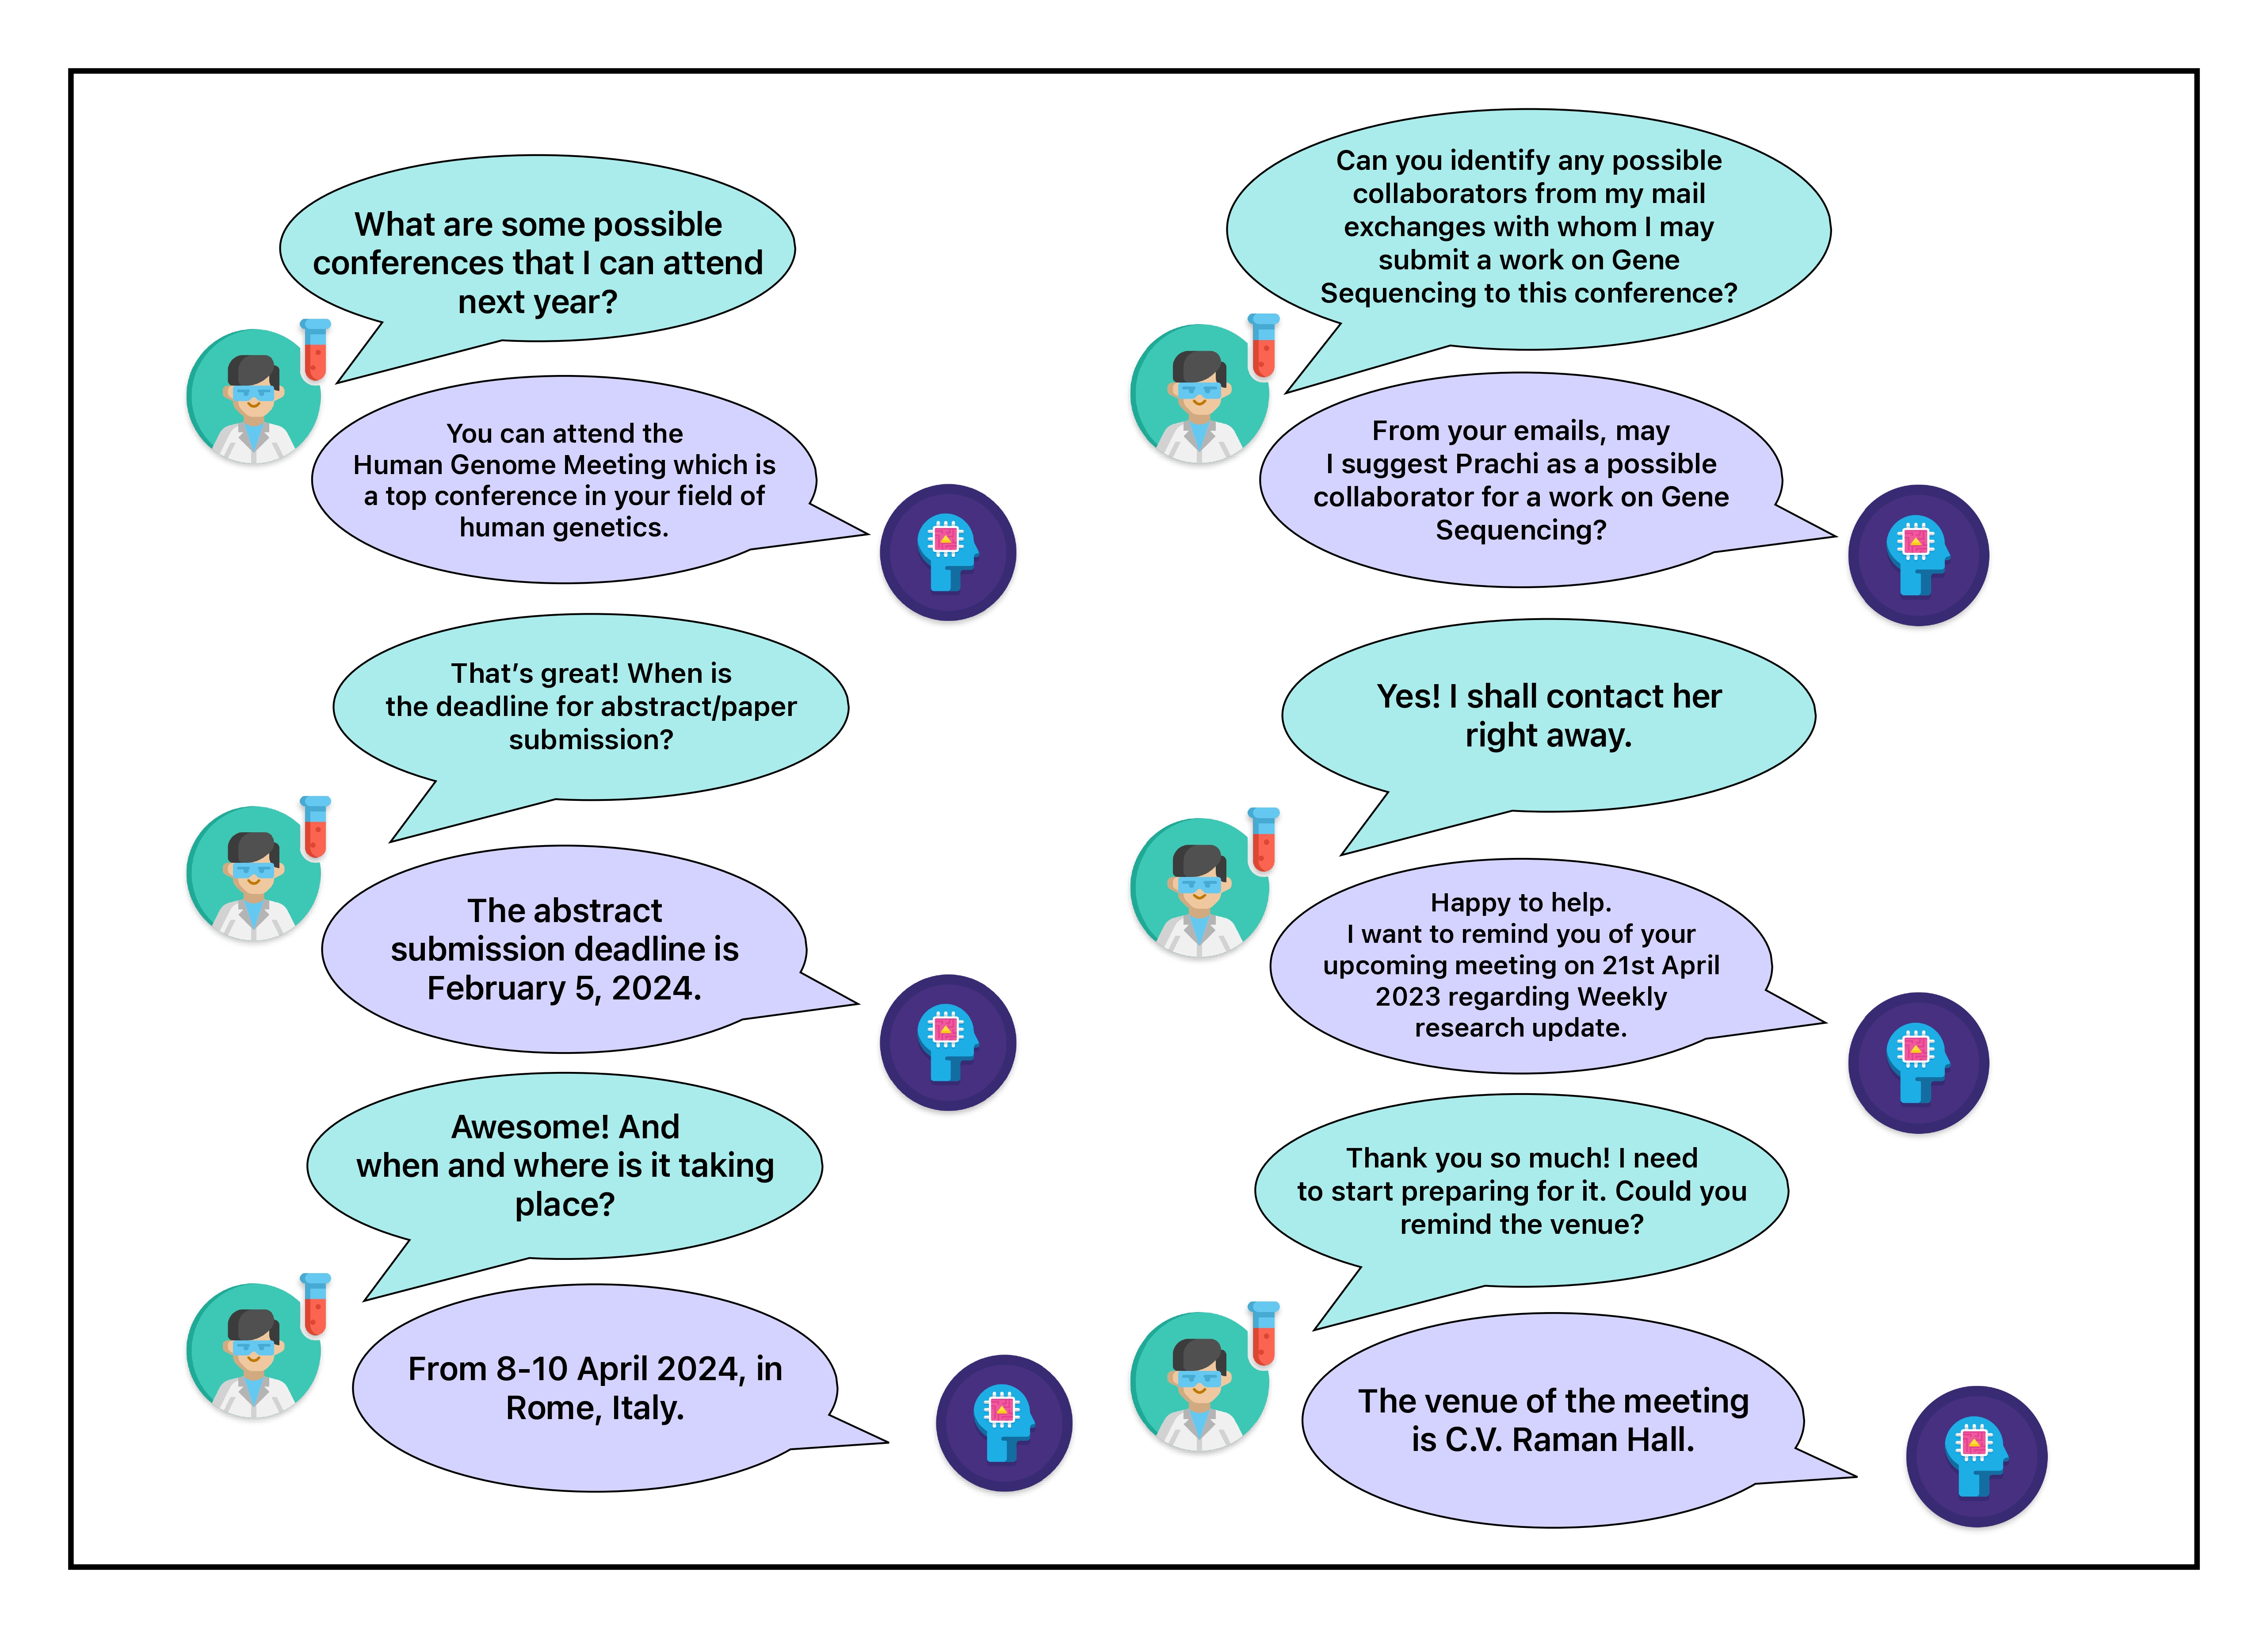
\includegraphics[width=0.8\textwidth]{submissions/Sudakshina2023/figs/PRKG_Interaction.jpg}
    \caption{An interaction between Vinay and the smart virtual agent who has access to Vinay's PRKG.}
    \label{fig:prkgInteraction}
\end{figure}

\section{Interacting with the PRKG} \label{prantika_sec:interact}
The potential of a PRKG can be fully realized only when a user can interact with it in order to make their daily research life more manageable. As observed in Section \ref{prantika_sec:requirements}, the owner of a PRKG will have frequent questions on topics like details of research papers read by them, upcoming meetings and summaries of past ones attended and research grants. In order to interact with the PRKG to access its stored knowledge, the owner will approach the smart virtual agent by asking the required questions.
Questions to the agent may be direct, whose response can be found in the KG with a simple database search. For example, Vinay, the owner of the PRKG in figure \ref{fig:prkg}, can ask questions regarding his upcoming engagements like, ``\textit{Where will the meeting on my weekly research update be held on 21st this month? Also, could you confirm the time of the meeting?}`` This is a fairly straightforward question that the agent will be able to respond to without any added inference. Some questions, however, may not be so direct for the agent. Questions like ``\textit{Can you identify a possible collaborator from the people I have been exchanging emails with regarding gene-sequencing?}``. The agent will have to go through all possible mail threads with the subject or summary with \textit{gene-sequencing} in it and identify and rank possible collaborators for Vinay. Once deduced, the agent may add this information to the PRKG. The agent may be directed to add, delete or modify inferred entities and relations on a routine basis, even before being prompted to do so, such that the PRKG remains updated. The agent may also remind the owner about upcoming scheduled events, submission deadlines, and to reply to a potentially important email as identified by the agent. A sample conversation between Vinay and the agent is shown in Figure \ref{fig:prkgInteraction}.

A PRKG holds significant relevance even when Large Language Models (LLMs), such as ChatGPT developed by OpenAI\footnote{\url{https://openai.com/chatgpt}} and LLaMa by Meta\cite{touvron2023llama}, have become widely popular for their ability to accurately follow user instructions and perform tasks such as question-answering, summarization, translation, and recommendation. The following issues with LLMs make their use particularly challenging:
\begin{itemize}
    \item \textit{Hallucinations:} LLMs have gained a reputation for generating false and unreliable responses, commonly known as hallucinations when faced with questions or prompts regarding unfamiliar knowledge not encountered during training \cite{ji2023surveyHallucination}. This drawback can pose significant risks in domains that demand precise information, like medicine \cite{beutel2023artificial} and law \cite{sun2023short}. In contrast, question-answering based on PRKGs can provide reliable information due to the specificity and ability to update the stored information, unlike LLMs trained on fixed data. Leveraging external knowledge about a user in the form of a PRKG can significantly enhance an LLM's capability to provide accurate and personalized responses, eliminating the need to predict or generate unreliable answers  \cite{peng2023check}. 

    \item \textit{Privacy concerns:} If a user provides personal information in the prompts with which they interact with the publicly available LLMs, it might end up into the training dataset of the LLM. Researchers have observed that it is possible to extract the training data by manipulating the LLM into sharing it, and this can lead to privacy breach attacks \cite{carlini2021extracting, nasr2023scalable}. 
    In contrast, a PRKG  offers transparency by granting users complete access and control over their stored data, empowering users with more agency over their personal information. One can also build LLM-based dialog systems that access the PRKG at response generation time, thereby harnessing the strengths of both LLMs and knowledge graphs.
\end{itemize} 

\section{Future Research Directions} \label{prantika_sec:future}
The \textit{personal} aspect of PRKGs introduces many challenges and opportunities in their  design, implementation, and evaluation. 
The first challenge relates to the composition of a PRKG. Consider any constituent KG like a Document KG or Email KG: even if the user identifies the documents or emails to be considered for the PRKG, it is unclear which entities and relations should be extracted for curation. The PRKG designer may specify a small default set of entities and relations (or ontology) that a researcher might be interested in (as we have done above), and allow the PRKG owner to extend it. Additionally, a machine learning algorithm in the PRKG editor might learn to suggest potential entities and relations to be extracted. Entity disambiguation is needed to link multiple mentions of the same entity like a collaborator or a journal. Entity disambiguation would be challenging for named entities that occur rarely in the user's data and are also uncommon in the external world. The lack of open datasets makes research in this area very difficult. Future work should organize community efforts to build datasets to catalyze the design and implementation of PRKGs. We also believe that more KGs can be conceived as components of the PRKG. For example, knowledge extracted from photographs captured by the scientist at conferences and meetings could form the basis for a new personal KG that helps to preserve and retrieve connected memories \cite{kottur2022navigating}.

Evaluation of a PRKG is another challenging area that is hardly explored. Since the personal data and expectations on what should go into a PRKG vary widely across researchers (based on their domain, seniority, etc.), evaluation strategies should be carefully designed keeping the PRKG owner in the loop. A closely related problem is the evaluation of a PRKG-based smart virtual agent: Can it understand and satisfy the user's information needs? Does it provide pro-active suggestions to the user? It is also desirable that the agent's responses are accompanied with explanations.  

A PRKG contains personal and sensitive information of its owner. So it should be securely stored whether on the user's local device or in the cloud. 
A PRKG contains information related to the research activities of its owner. Therefore, the PRKG owner might like to share parts of the PRKG with their collaborators including students.  
Similarly, the PRKG owner could personalize various services like recommendation systems and search engines with the PRKG. This raises the question about how the PRKG owner can grant access to other users and applications without privacy leaks and without allowing unintended modification of information. Investigation of these aspects may be informed by the existing research on privacy-preserving KGs \cite{chen2020survey,purificato2021dynamic}.

\section{Conclusion} \label{prantika_sec:conclusion}
We have discussed the notion of personal research knowledge graphs, which are employed to store the information that is personally relevant to a researcher. Through interviews with multiple scientists, we identified their requirements for personal data management and put forth a design for PRKGs to capture the necessary knowledge. We acknowledged several challenges in the design, implementation and evaluation of PRKGs. Nevertheless, if done right, they can be immensely valuable in building applications that bring order to the information chaos and alleviate the overload that the researcher experiences. This, in turn, can translate to better productivity, hightened job  satisfaction and improved work-life balance. 


\bibliographystyle{plain} 
\bibliography{submissions/Sudakshina2023/ref}


\end{document}